\documentclass[11pt]{article}

\usepackage[T1]{fontenc}
\usepackage{lmodern}
\usepackage[letterpaper,margin=0.68in]{geometry}
\usepackage{booktabs}
\usepackage{amsmath}
\usepackage{graphicx}
\usepackage{threeparttable}
\usepackage{caption}
\usepackage{float}
\usepackage{microtype}

\captionsetup{font=small,labelfont=bf,justification=centering}
\setlength{\parindent}{0pt}
\setlength{\parskip}{4pt}
\def\sym#1{\ifmmode^{#1}\else\(^{#1}\)\fi}

\begin{document}

\begin{center}
  {\Large\bfseries CEI and CCEI Results}\par
  \vspace{2pt}
  {\small Pooled baseline and endline sample}
\end{center}

\vspace{4pt}

\begin{table}[H]
\centering
\caption{Group CCEI and Group CEI}
\label{tab:cei-ccei-separate}
\begin{threeparttable}
\footnotesize
\renewcommand{\arraystretch}{0.86}
\setlength{\tabcolsep}{7.5pt}
\begin{tabular}{lcccc}
\toprule
&\multicolumn{1}{c}{(1)}&\multicolumn{1}{c}{(2)}&\multicolumn{1}{c}{(3)}&\multicolumn{1}{c}{(4)}\\
\midrule
\multicolumn{5}{l}{\textit{Panel A: Group CCEI -- OLS}}\\
$\text{CCEI}_{\text{max},gt}$&    0.127        &    0.108        &    0.113        &    0.060        \\
                &  (0.098)        &  (0.096)        &  (0.094)        &  (0.120)        \\
$\text{CCEI}_{\text{min},gt}$&    0.234\sym{**}&    0.224\sym{**}&    0.181\sym{**}&    0.127\sym{**}\\
                &  (0.045)        &  (0.045)        &  (0.038)        &  (0.045)        \\
\midrule
N               &     1304        &     1304        &     1304        &     1304        \\
R-squared       &    0.166        &    0.182        &    0.204        &    0.645        \\

\midrule
\multicolumn{5}{l}{\textit{Panel B: Group CEI -- OLS}}\\
$\text{CCEI}_{\text{max},gt}$&    0.252\sym{**}&    0.250\sym{**}&    0.234\sym{**}&    0.202\sym{*} \\
                &  (0.093)        &  (0.089)        &  (0.086)        &  (0.099)        \\
$\text{CCEI}_{\text{min},gt}$&    0.007        &    0.006        &   -0.026        &   -0.085\sym{*} \\
                &  (0.023)        &  (0.024)        &  (0.026)        &  (0.042)        \\
\midrule
N               &     1304        &     1304        &     1304        &     1304        \\
R-squared       &    0.083        &    0.102        &    0.116        &    0.582        \\

\midrule
\multicolumn{5}{l}{\textit{Panel C: Group CCEI -- fractional-response APEs}}\\
$\text{CCEI}_{\text{max},gt}$&    0.077        &    0.060        &    0.082\sym{+} &    0.029        \\
                &  (0.054)        &  (0.051)        &  (0.049)        &  (0.082)        \\
$\text{CCEI}_{\text{min},gt}$&    0.176\sym{**}&    0.170\sym{**}&    0.138\sym{**}&    0.094\sym{**}\\
                &  (0.023)        &  (0.023)        &  (0.022)        &  (0.032)        \\
\midrule
N               &     1304        &     1304        &     1304        &     1304        \\

\midrule
\multicolumn{5}{l}{\textit{Panel D: Group CEI -- fractional-response APEs}}\\
$\text{CCEI}_{\text{max},gt}$&    0.176\sym{**}&    0.179\sym{**}&    0.164\sym{**}&    0.132\sym{+} \\
                &  (0.056)        &  (0.053)        &  (0.049)        &  (0.068)        \\
$\text{CCEI}_{\text{min},gt}$&    0.009        &    0.009        &   -0.022        &   -0.069\sym{*} \\
                &  (0.021)        &  (0.023)        &  (0.025)        &  (0.035)        \\
\midrule
N               &     1304        &     1304        &     1304        &     1304        \\
\bottomrule

\end{tabular}
\begin{tablenotes}[flushleft]
\scriptsize
\item \textit{Notes:} Each observation is a pair-wave. Panels A and B report OLS coefficients. Panels C and D report average partial effects (APEs). Columns (1)--(3) of Panels C and D use fractional logit. Column (4) uses the strictly exogenous correlated-random-effects fractional probit QMLE of Papke and Wooldridge (2008), with full controls, pair means of wave-varying covariates, a wave intercept, and class fixed effects. Columns (1)--(3) absorb class fixed effects; Column (4) of Panels A and B instead absorbs pair fixed effects. Standard errors are clustered by class. $+\ p<0.10$, $*\ p<0.05$, $**\ p<0.01$.
\end{tablenotes}
\end{threeparttable}
\end{table}

\clearpage

\begin{table}[H]
\centering
\caption{Joint Group CEI and Group CCEI Classification}
\label{tab:cei-ccei-joint}
\begin{threeparttable}
\small
\renewcommand{\arraystretch}{0.91}
\setlength{\tabcolsep}{7.5pt}
\begin{tabular}{lcccc}
\toprule
&\multicolumn{1}{c}{(1)}&\multicolumn{1}{c}{(2)}&\multicolumn{1}{c}{(3)}&\multicolumn{1}{c}{(4)}\\
\midrule
Stable-weight vs. Pareto inefficient&                 &                 &                 &                 \\
CCEI max (0.1)  &    1.108\sym{**}&    1.061\sym{**}&    1.035\sym{**}&    0.498\sym{+} \\
                &  (0.232)        &  (0.228)        &  (0.222)        &  (0.278)        \\
CCEI min (0.1)  &    0.059        &    0.031        &    0.015        &   -0.070        \\
                &  (0.065)        &  (0.069)        &  (0.081)        &  (0.117)        \\
Varying-weight vs. Pareto inefficient&                 &                 &                 &                 \\
CCEI max (0.1)  &    0.266\sym{+} &    0.271\sym{+} &    0.188        &    0.173        \\
                &  (0.149)        &  (0.152)        &  (0.159)        &  (0.224)        \\
CCEI min (0.1)  &   -0.182\sym{**}&   -0.187\sym{**}&   -0.202\sym{**}&   -0.368\sym{**}\\
                &  (0.062)        &  (0.065)        &  (0.073)        &  (0.116)        \\
\midrule
Pair-wave observations&     1304        &     1304        &     1304        &      834        \\
Pairs           &      652        &      652        &      652        &      417        \\
Pseudo R-squared&    0.097        &    0.118        &    0.139        &    0.222        \\
\bottomrule

\end{tabular}
\begin{tablenotes}[flushleft]
\scriptsize
\item \textit{Notes:} Multinomial-logit coefficients are reported relative to the Pareto-inefficient category, defined as group CEI $<1$. Stable-weight denotes CEI $=1$ and CCEI $=1$; varying-weight denotes CEI $=1$ and CCEI $<1$. CCEI coefficients correspond to a 0.1 increase. Columns (1)--(3) absorb class fixed effects and sequentially add the controls used in Table 1. Column (4) uses conditional pair fixed effects and therefore retains 417 pairs whose category changes across waves. Its pseudo $R^2$ is based on the conditional likelihood and is not directly comparable to Columns (1)--(3). Standard errors are clustered by class. $+\ p<0.10$, $*\ p<0.05$, $**\ p<0.01$.
\end{tablenotes}
\end{threeparttable}
\end{table}

\vspace{3pt}

\begin{figure}[H]
\centering
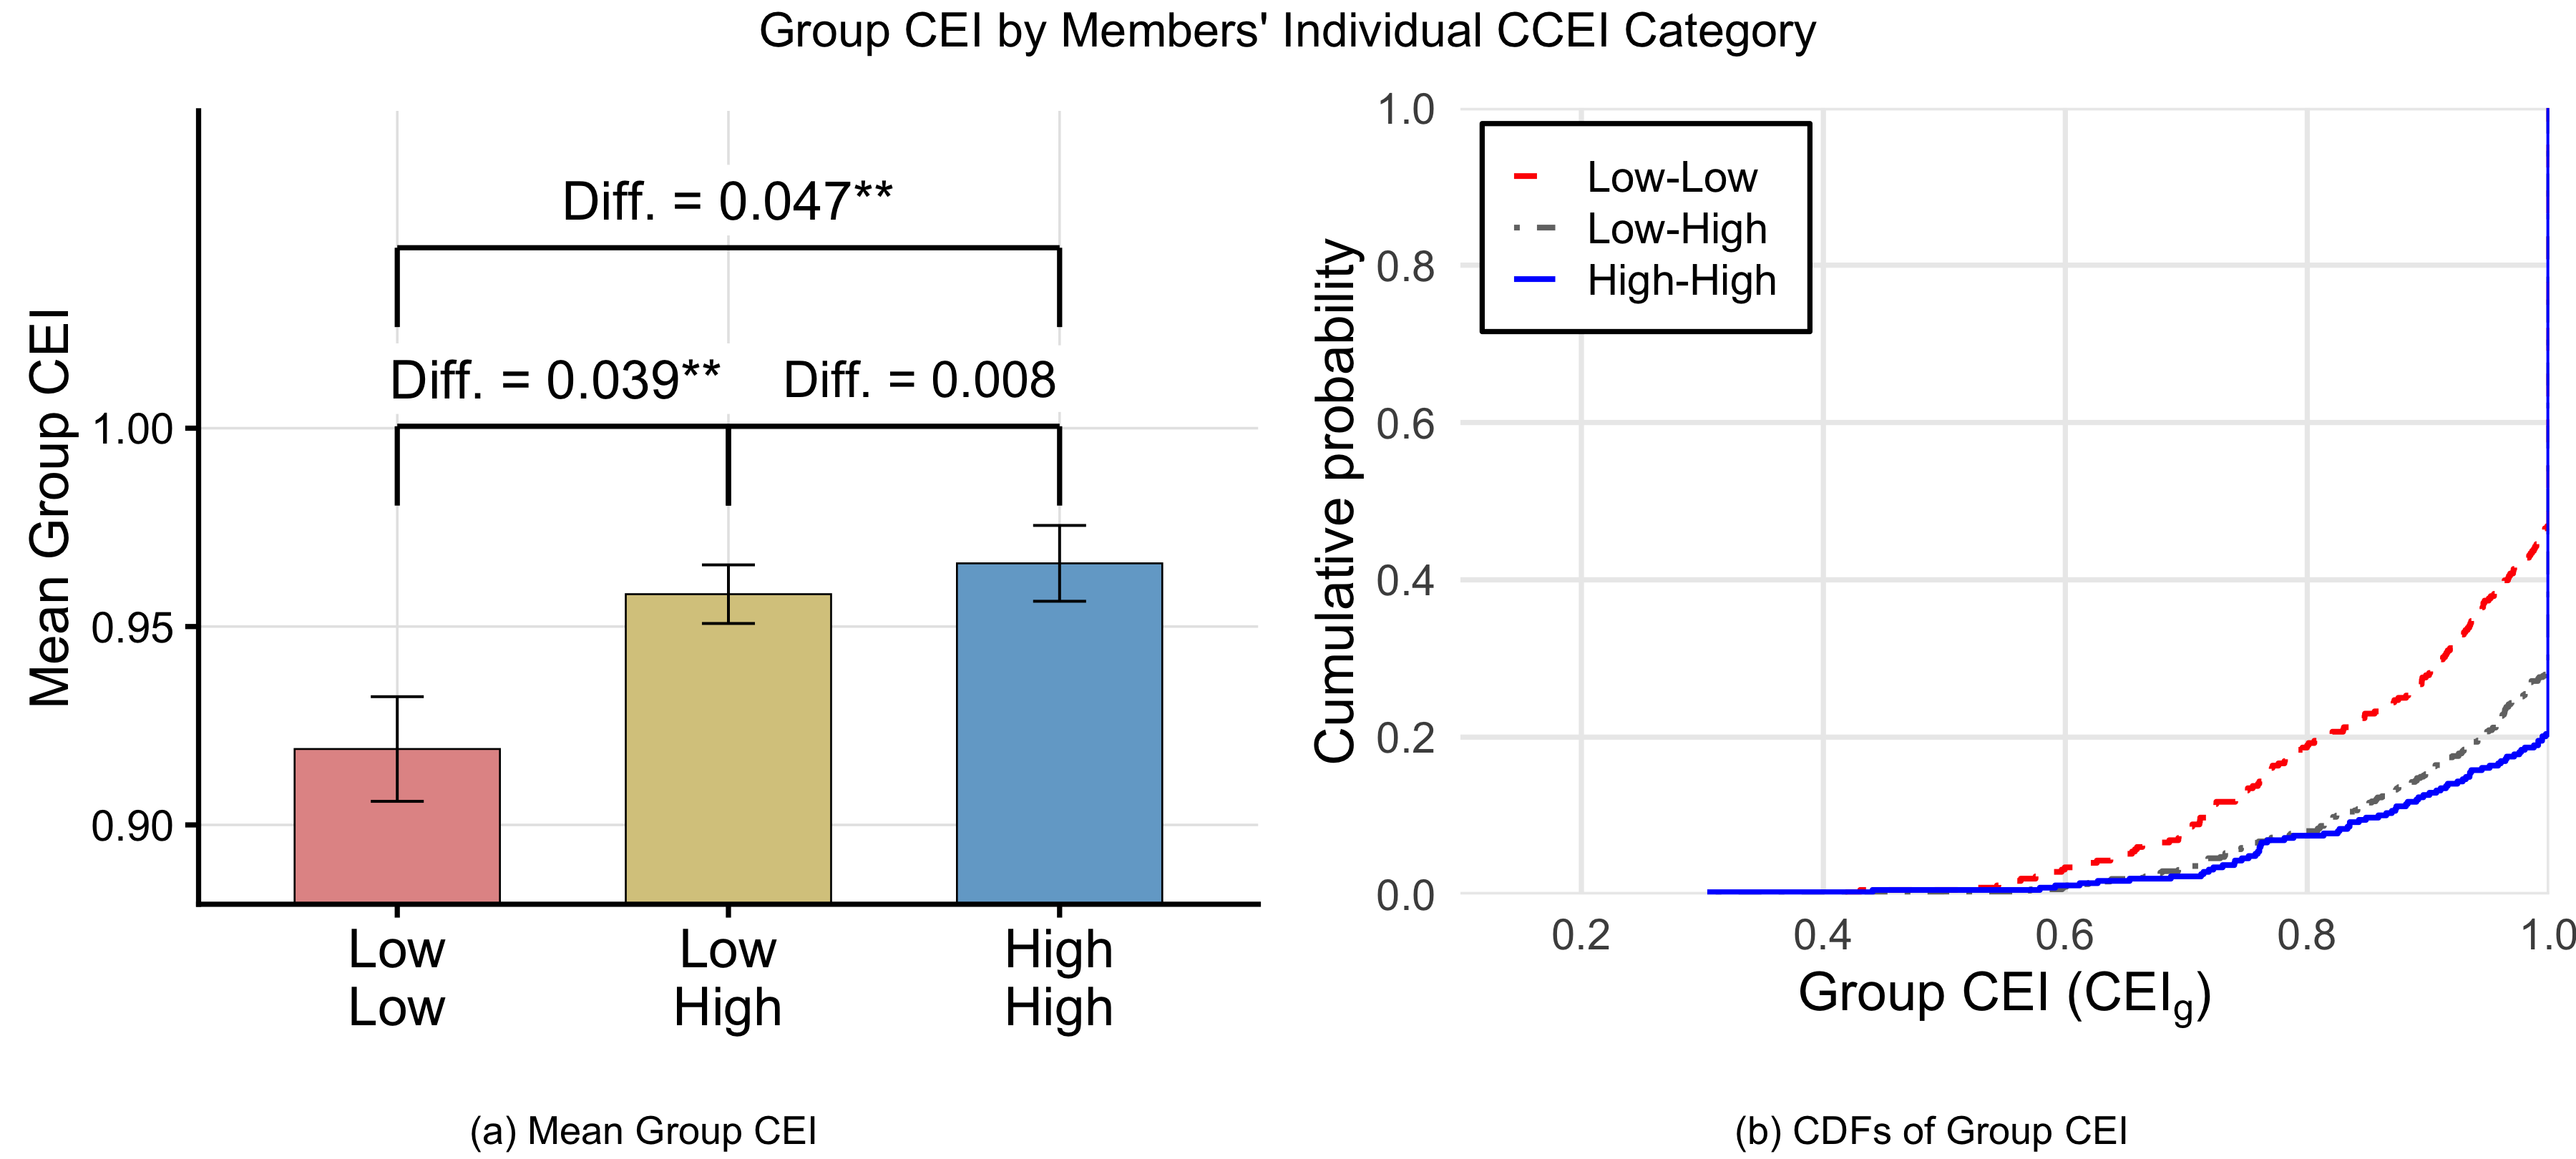
\includegraphics[width=0.96\textwidth]{results/figures/temp_cei_min_group_cei_by_member_ccei_category.png}
\caption{Group CEI by Members' Individual CCEI Category}
\label{fig:group-cei-member-ccei}
\begin{minipage}{0.96\textwidth}
\scriptsize
\textit{Notes:} Individual categories use the pooled median individual CCEI, with baseline and endline observations pooled. Bars report mean group CEI and 95\% confidence intervals. Difference labels report two-sample Welch tests. The category sample sizes are 348, 608, and 348 for Low-Low, Low-High, and High-High, respectively. $+\ p<0.10$, $*\ p<0.05$, $**\ p<0.01$.
\end{minipage}
\end{figure}

\clearpage

\begin{center}
  {\large\bfseries Alternative CCEI Parameterization}
\end{center}

\begin{table}[H]
\centering
\caption{Group CCEI and Group CEI - CCEI Maximum and Distance}
\label{tab:cei-ccei-separate-dist}
\begin{threeparttable}
\footnotesize
\renewcommand{\arraystretch}{0.86}
\setlength{\tabcolsep}{7.5pt}
\begin{tabular}{lcccc}
\toprule
&\multicolumn{1}{c}{(1)}&\multicolumn{1}{c}{(2)}&\multicolumn{1}{c}{(3)}&\multicolumn{1}{c}{(4)}\\
\midrule
\multicolumn{5}{l}{\textit{Panel A: Group CCEI -- OLS}}\\
$\text{CCEI}_{\text{max},gt}$&    0.362\sym{**}&    0.332\sym{**}&    0.293\sym{**}&    0.187\sym{+} \\
                &  (0.081)        &  (0.081)        &  (0.076)        &  (0.109)        \\
$\text{CCEI}_{\text{dist},gt}$&   -0.234\sym{**}&   -0.224\sym{**}&   -0.181\sym{**}&   -0.127\sym{**}\\
                &  (0.045)        &  (0.045)        &  (0.038)        &  (0.045)        \\
\midrule
N               &     1304        &     1304        &     1304        &     1304        \\
R-squared       &    0.166        &    0.182        &    0.204        &    0.645        \\

\midrule
\multicolumn{5}{l}{\textit{Panel B: Group CEI -- OLS}}\\
$\text{CCEI}_{\text{max},gt}$&    0.259\sym{**}&    0.256\sym{**}&    0.208\sym{*} &    0.117        \\
                &  (0.083)        &  (0.081)        &  (0.079)        &  (0.100)        \\
$\text{CCEI}_{\text{dist},gt}$&   -0.007        &   -0.006        &    0.026        &    0.085\sym{*} \\
                &  (0.023)        &  (0.024)        &  (0.026)        &  (0.042)        \\
\midrule
N               &     1304        &     1304        &     1304        &     1304        \\
R-squared       &    0.083        &    0.102        &    0.116        &    0.582        \\

\midrule
\multicolumn{5}{l}{\textit{Panel C: Group CCEI -- fractional-response APEs}}\\
$\text{CCEI}_{\text{max},gt}$&    0.252\sym{**}&    0.231\sym{**}&    0.220\sym{**}&    0.123\sym{+} \\
                &  (0.046)        &  (0.044)        &  (0.040)        &  (0.073)        \\
$\text{CCEI}_{\text{dist},gt}$&   -0.176\sym{**}&   -0.170\sym{**}&   -0.138\sym{**}&   -0.094\sym{**}\\
                &  (0.023)        &  (0.023)        &  (0.022)        &  (0.032)        \\
\midrule
N               &     1304        &     1304        &     1304        &     1304        \\

\midrule
\multicolumn{5}{l}{\textit{Panel D: Group CEI -- fractional-response APEs}}\\
$\text{CCEI}_{\text{max},gt}$&    0.185\sym{**}&    0.188\sym{**}&    0.142\sym{**}&    0.063        \\
                &  (0.048)        &  (0.044)        &  (0.043)        &  (0.066)        \\
$\text{CCEI}_{\text{dist},gt}$&   -0.009        &   -0.009        &    0.022        &    0.069\sym{*} \\
                &  (0.021)        &  (0.023)        &  (0.025)        &  (0.035)        \\
\midrule
N               &     1304        &     1304        &     1304        &     1304        \\
\bottomrule

\end{tabular}
\begin{tablenotes}[flushleft]
\scriptsize
\item \textit{Notes:} CCEI distance equals CCEI maximum minus CCEI minimum; larger values indicate greater within-pair disparity. The maximum coefficient therefore holds distance fixed. This is an exact reparameterization of Table 1, so fitted values, predictions, sample sizes, and fit statistics are unchanged. Panels A and B report OLS coefficients. Panels C and D report APEs. Columns (1)--(3) of Panels C and D use fractional logit. Column (4) uses the strictly exogenous correlated-random-effects fractional probit QMLE of Papke and Wooldridge (2008), with full controls, pair means of wave-varying covariates, a wave intercept, and class fixed effects. Columns (1)--(3) absorb class fixed effects; Column (4) of Panels A and B instead absorbs pair fixed effects. Standard errors are clustered by class. $+\ p<0.10$, $*\ p<0.05$, $**\ p<0.01$.
\end{tablenotes}
\end{threeparttable}
\end{table}

\clearpage

\begin{table}[H]
\centering
\caption{Joint Group CEI and Group CCEI Classification - CCEI Maximum and Distance}
\label{tab:cei-ccei-joint-dist}
\begin{threeparttable}
\footnotesize
\renewcommand{\arraystretch}{0.95}
\setlength{\tabcolsep}{9pt}
\begin{tabular}{lcccc}
\toprule
&\multicolumn{1}{c}{(1)}&\multicolumn{1}{c}{(2)}&\multicolumn{1}{c}{(3)}&\multicolumn{1}{c}{(4)}\\
\midrule
Stable-weight vs. Pareto inefficient&                 &                 &                 &                 \\
CCEI max (0.1)  &    1.167\sym{**}&    1.092\sym{**}&    1.050\sym{**}&    0.428\sym{+} \\
                &  (0.211)        &  (0.210)        &  (0.207)        &  (0.246)        \\
CCEI distance (0.1)&   -0.059        &   -0.031        &   -0.015        &    0.070        \\
                &  (0.065)        &  (0.069)        &  (0.081)        &  (0.117)        \\
Varying-weight vs. Pareto inefficient&                 &                 &                 &                 \\
CCEI max (0.1)  &    0.084        &    0.084        &   -0.014        &   -0.195        \\
                &  (0.124)        &  (0.124)        &  (0.139)        &  (0.230)        \\
CCEI distance (0.1)&    0.182\sym{**}&    0.187\sym{**}&    0.202\sym{**}&    0.368\sym{**}\\
                &  (0.062)        &  (0.065)        &  (0.073)        &  (0.116)        \\
\midrule
Pair-wave observations&     1304        &     1304        &     1304        &      834        \\
Pairs           &      652        &      652        &      652        &      417        \\
Pseudo R-squared&    0.097        &    0.118        &    0.139        &    0.222        \\
\bottomrule

\end{tabular}
\begin{tablenotes}[flushleft]
\scriptsize
\item \textit{Notes:} CCEI distance equals CCEI maximum minus CCEI minimum; larger values indicate greater within-pair disparity. The maximum coefficient therefore holds distance fixed. This is an exact reparameterization of Table 2, so fitted values, predictions, sample sizes, and fit statistics are unchanged. Multinomial-logit coefficients are relative to the Pareto-inefficient category, defined as group CEI $<1$. Stable-weight denotes CEI $=1$ and CCEI $=1$; varying-weight denotes CEI $=1$ and CCEI $<1$. CCEI coefficients correspond to a 0.1 increase. Columns (1)--(3) absorb class fixed effects and sequentially add the controls used in Table 1. Column (4) uses conditional pair fixed effects and retains 417 pairs whose category changes across waves. Its pseudo $R^2$ is based on the conditional likelihood and is not directly comparable to Columns (1)--(3). Standard errors are clustered by class. $+\ p<0.10$, $*\ p<0.05$, $**\ p<0.01$.
\end{tablenotes}
\end{threeparttable}
\end{table}

\end{document}
